% !TEX TS-program = lualatex
% !BIB TS-program = biber
%\documentclass[handout]{beamer}
\documentclass{beamer}
\newcommand{\misoclasstinytitleslide}{Partially based on material by:  Rob Fergus, Nikhil Srivastava,\\[-1em] 
Yiannis Koutis, Joshua Batson, Daniel Spielman}
%{Partially based on material by:  Branislav Kveton,  \\[-1em]  Partha Niyogi, Rob Fergus}
\newcommand{\misoclassdate}{}
\input{../common/misomva}
\usepackage{verbatim}
\usepackage{listings}
\usepackage[customcolors]{hf-tikz}
\usepackage{color}
\usepackage{cancel}
%\usepackage[defaultmono]{droidmono}
\newcommand{\nbskip}{\vspace{-\baselineskip}}
%\newcommand{\hbskip}{\vspace{.5\baselineskip}}
\newcommand{\nhbskip}{\vspace{-.5\baselineskip}}

\definecolor{mygreen}{rgb}{0,0.6,0}
\definecolor{mygray}{rgb}{0.5,0.5,0.5}
\definecolor{mymauve}{rgb}{0.58,0,0.82}

\definecolor{Code}{rgb}{0,0,0}
\definecolor{Decorators}{rgb}{0.5,0.5,0.5}
\definecolor{Numbers}{rgb}{0.5,0,0}
\definecolor{MatchingBrackets}{rgb}{0.25,0.5,0.5}
\definecolor{Keywords}{rgb}{0,0,1}
\definecolor{self}{rgb}{0,0,0}
\definecolor{Strings}{rgb}{0,0.63,0}
\definecolor{Comments}{rgb}{0,0.63,1}
\definecolor{Backquotes}{rgb}{0,0,0}
\definecolor{Classname}{rgb}{0,0,0}
\definecolor{FunctionName}{rgb}{0,0,0}
\definecolor{Operators}{rgb}{0,0,0}
\definecolor{Background}{rgb}{0.98,0.98,0.98}

\lstset{ %
backgroundcolor=\color{white},   % choose the background color; you must add \usepackage{color} or \usepackage{xcolor}
basicstyle=\fdmfamily\footnotesize,        % the size of the fonts that are used for the code
breakatwhitespace=false,         % sets if automatic breaks should only happen at whitespace
breaklines=true,                 % sets automatic line breaking
captionpos=b,                    % sets the caption-position to bottom
commentstyle=\color{mygreen},    % comment style
deletekeywords={\dots},            % if you want to delete keywords from the given language
escapeinside={\%*}{*)},          % if you want to add LaTeX within your code
extendedchars=true,              % lets you use non-ASCII characters; for 8-bits encodings only, does not work with UTF-8
frame=single,	                   % adds a frame around the code
keepspaces=true,                 % keeps spaces in text, useful for keeping indentation of code (possibly needs columns=flexible)
language=Python,                 % the language of the code
% Comments
commentstyle=\color{Comments}\slshape,
% Strings
stringstyle=\color{Strings},
morecomment=[s][\color{Strings}]{"""}{"""},
morecomment=[s][\color{Strings}]{'''}{'''},
% keywords
morekeywords={import,from,class,def,for,while,if,is,in,elif,else,not,and,or,print,break,continue,return,True,False,None,access,as,,del,except,exec,finally,global,import,lambda,pass,print,raise,try,assert},
keywordstyle={\color{Keywords}\bfseries},
% additional keywords
morekeywords={[2]@invariant},
keywordstyle={[2]\color{Decorators}\slshape},
emph={self},
emphstyle={\color{self}\slshape},
otherkeywords={*,\dots},            % if you want to add more keywords to the set
numbers=left,                    % where to put the line-numbers; possible values are (none, left, right)
numbersep=5pt,                   % how far the line-numbers are from the code
numberstyle=\tiny\color{mygray}, % the style that is used for the line-numbers
rulecolor=\color{black},         % if not set, the frame-color may be changed on line-breaks within not-black text (e.g. comments (green here))
showspaces=false,                % show spaces everywhere adding particular underscores; it overrides 'showstringspaces'
showstringspaces=false,          % underline spaces within strings only
showtabs=false,                  % show tabs within strings adding particular underscores
stepnumber=1,                    % the step between two line-numbers. If it's 1, each line will be numbered
tabsize=2,	                   % sets default tabsize to 2 spaces
title=\lstname                   % show the filename of files included with \lstinputlisting; also try caption instead of title
}


\newcommand{\consindent}[1]{
    \begin{itemize}
        \item[{
\includegraphics[height=0.7\baselineskip]{../img/arrow_list}}] #1
    \end{itemize}
}


%%% part daniele
\usepackage{etex}
\TPshowboxesfalse
\textblockorigin{0mm}{0mm}

\definecolor{rouge1}{RGB}{226,0,38}  % red P
\definecolor{orange1}{RGB}{243,154,38}  % orange P
\definecolor{jaune}{RGB}{254,205,27}  % jaune P
\definecolor{blanc}{RGB}{255,255,255} % blanc P

\definecolor{rouge2}{RGB}{230,68,57}  % red S
\definecolor{orange2}{RGB}{236,117,40}  % orange S
\definecolor{taupe}{RGB}{134,113,127} % taupe S
\definecolor{gris}{RGB}{91,94,111} % gris S
\definecolor{bleu1}{RGB}{38,109,131} % bleu S
\definecolor{bleu2}{RGB}{28,50,114} % bleu S
\definecolor{vert1}{RGB}{133,146,66} % vert S
\definecolor{vert3}{RGB}{20,200,66} % vert S
\definecolor{vert2}{RGB}{157,193,7} % vert S
\definecolor{darkyellow}{RGB}{233,165,0}  % orange S
\definecolor{lightgray}{rgb}{0.9,0.9,0.9}
\definecolor{darkgray}{rgb}{0.6,0.6,0.6}

\setbeamertemplate{navigation symbols}{}
\setbeamertemplate{blocks}[rounded]
\setbeamercolor{block title}{bg=bleu2,fg=white}%bg=background, fg= foreground
\setbeamercolor{block body}{bg=lightgray}%bg=background, fg= foreground

\renewcommand{\sfdefault}{lmss}
\sffamily

%\newcommand{\ycol}[1]{\textcolor{darkyellow}{\textit{#1}}}

\newcommand{\rcolb}[1]{\textcolor{red}{\textit{\textbf{#1}}}}
\newcommand{\gcolb}[1]{\textcolor{vert3}{\textit{\textbf{#1}}}}
\newcommand{\bcolb}[1]{\textcolor{blue}{\textit{\textbf{#1}}}}
\newcommand{\ycolb}[1]{\textcolor{darkyellow}{\textit{\textbf{#1}}}}

\newcommand{\eqrcol}[1]{\textcolor{red}{#1}}
\newcommand{\eqgcol}[1]{\textcolor{vert3}{#1}}
\newcommand{\eqbcol}[1]{\textcolor{blue}{#1}}
\newcommand{\eqrcolb}[1]{\textcolor{red!70}{\mathbf{#1}}}
\newcommand{\eqgcolb}[1]{\textcolor{vert3!70}{\mathbf{#1}}}
\newcommand{\eqbcolb}[1]{\textcolor{blue!70}{\mathbf{#1}}}
\newcommand{\eqycol}[1]{\textcolor{darkyellow}{#1}}

%\newcommand{\otoprule}{\midrule[\heavyrulewidth]}

\colorlet{redp}{red!20} % vert S
\colorlet{greenp}{vert3!20} % vert S
\colorlet{bluep}{blue!20} % vert S

\usepackage{adjustbox}

% Highlight and cancel commands are defined in misomva.tex

\newcommand{\bookboxx}[1]{
\par\medskip\noindent
\framebox[\columnwidth]{
\begin{minipage}{0.98\columnwidth} {\par\smallskip#1\par\smallskip} \end{minipage} } \par\medskip }

\setbeamersize{text margin left=1cm,text margin right=1cm}
\tikzstyle{every picture}+=[remember picture]

\newcommand{\incarrow}{{
\includegraphics[height=0.7\baselineskip]{../img/arrow_list}}}
\newcommand{\consarrow}{{\hspace*{.1pt} 
\includegraphics[height=0.7\baselineskip]{../img/arrow_list}}\;}

% Change margins for slides
\newenvironment{changemargin}[2]{% 
  \begin{list}{}{% 
    \setlength{\topsep}{0pt}% 
    \setlength{\leftmargin}{#1}% 
    \setlength{\rightmargin}{#2}% 
    \setlength{\listparindent}{\parindent}% 
    \setlength{\itemindent}{\parindent}% 
    \setlength{\parsep}{\parskip}% 
  }% 
  \item[]}{\end{list}} 


\newcommand{\ie}{i.e.\xspace}
\newcommand{\eg}{e.g.\xspace}

\newcommand{\greycite}[1]{{\small \textcolor{gray}{\cite{#1}}}}
%%%

\begin{document}
% Topic-specific title slide

\newcommand{\topictitle}{Cut Graph Sparsifiers}

\newcommand{\topicsubtitle}{Benczur-Karger Algorithm}
\renewcommand{\misoclasstinytitleslide}{Partially based on material by:  Rob Fergus, Nikhil Srivastava,\\[-1em] Yiannis Koutis, Joshua Batson, Daniel Spielman}

\MakeTopicSlide

\begin{frame}
\frametitle{Cut Graph Sparsifiers}
%\moveb \pause 
Define $G$ and $H$ are \emphcol{$(1\pm\eps)$-cut similar}  when $\forall S$
\[
\alert{(1-\eps)}\text{cut}_{H}(S)  \leq  \text{cut}_{G}(S) \leq \alert{(1+\eps)}\text{cut}_{H}(S)
\]
\moveb \pause 
\questionbox{Why did they care?} \pause faster mincut/maxflow
\moveb \pause 
\questionbox{Is this always possible?} \pause 
\yellbox{Bencz\' ur and Karger (1996): Yes!}
\\ \smallskip
 $\forall \eps~\exists~ (1+\eps)$-cut similar $H$
with $\cO(n \log n/ \eps^2)$  edges s.t. $E_H \subseteq E$
and computable in  $\cO(m \log^3 n + m\log n /\eps^2)$ time 
\notecol{\tiny $n$ nodes, $m$ edges} 
\end{frame}
%%%%%%%%%%%%%%%%%%%%%%%%%%%%
\begin{frame}[t]
\frametitle{Cut Graph Sparsifiers}
%\frametitle{Graph Sparsification: What is \alert{good} sparse?}
\begin{center}
\qquad $G =$ \emphcol{$K_n$} \hskip 4cm $H = $ \emphcol{$d$-regular}  (random)
% TikZ replacement for sriva3 - Complete K_6 vs sparse graph
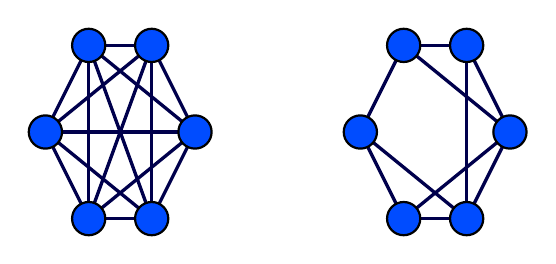
\begin{tikzpicture}[
    vertex/.style={circle, fill=blue!70!cyan, draw=black, line width=0.8pt, minimum size=12pt, inner sep=0pt},
    edge/.style={draw=blue!30!black, line width=1.2pt}
]
    \def\xsep{4}
    % LEFT: Complete K_6
    \coordinate (L1) at (-0.4, 1.1);  \coordinate (L2) at (0.4, 1.1);
    \coordinate (L3) at (-0.95, 0);   \coordinate (L4) at (0.95, 0);
    \coordinate (L5) at (-0.4, -1.1); \coordinate (L6) at (0.4, -1.1);
    \draw[edge] (L1)--(L2); \draw[edge] (L1)--(L3); \draw[edge] (L1)--(L4);
    \draw[edge] (L1)--(L5); \draw[edge] (L1)--(L6); \draw[edge] (L2)--(L3);
    \draw[edge] (L2)--(L4); \draw[edge] (L2)--(L5); \draw[edge] (L2)--(L6);
    \draw[edge] (L3)--(L4); \draw[edge] (L3)--(L5); \draw[edge] (L3)--(L6);
    \draw[edge] (L4)--(L5); \draw[edge] (L4)--(L6); \draw[edge] (L5)--(L6);
    \node[vertex] at (L1) {}; \node[vertex] at (L2) {};
    \node[vertex] at (L3) {}; \node[vertex] at (L4) {};
    \node[vertex] at (L5) {}; \node[vertex] at (L6) {};
    % RIGHT: Sparse graph
    \coordinate (R1) at (\xsep-0.4, 1.1);  \coordinate (R2) at (\xsep+0.4, 1.1);
    \coordinate (R3) at (\xsep-0.95, 0);   \coordinate (R4) at (\xsep+0.95, 0);
    \coordinate (R5) at (\xsep-0.4, -1.1); \coordinate (R6) at (\xsep+0.4, -1.1);
    \draw[edge] (R1)--(R2); \draw[edge] (R1)--(R3); \draw[edge] (R2)--(R4);
    \draw[edge] (R3)--(R5); \draw[edge] (R4)--(R6); \draw[edge] (R5)--(R6);
    \draw[edge] (R3)--(R6); \draw[edge] (R4)--(R5);
    \draw[edge] (R1)--(R4); \draw[edge] (R2)--(R6);
    \node[vertex] at (R1) {}; \node[vertex] at (R2) {};
    \node[vertex] at (R3) {}; \node[vertex] at (R4) {};
    \node[vertex] at (R5) {}; \node[vertex] at (R6) {};
\end{tikzpicture}
\pause 
\questionbox{How many edges?}
\moveb \pause 
$ |E_G| =  \cO(n^2) $ \hfil \pause  
$ |E_H| =  \cO(dn) $
\end{center}
\end{frame}
%%%%%%%%%%%%%%%%%%%%%%%%%%%%
\begin{frame}[t]
\frametitle{Cut Graph Sparsifiers}
%\frametitle{Graph Sparsification: What is \alert{good} sparse?}
\begin{center}
\qquad $G =$ \emphcol{$K_n$} \hskip 4cm $H = $ \emphcol{$d$-regular}  (random)
% TikZ replacement for sriva4 - K_6 vs sparse graph with cut (blue edges)
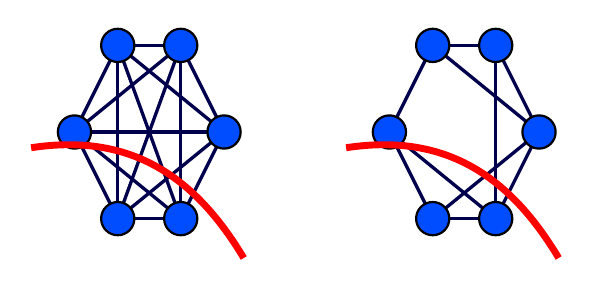
\begin{tikzpicture}[
    vertex/.style={circle, fill=blue!70!cyan, draw=black, line width=0.8pt, minimum size=12pt, inner sep=0pt},
    edge/.style={draw=blue!30!black, line width=1.2pt},
    cut/.style={draw=red, line width=2.5pt}
]
    \def\xsep{4}
    % LEFT: Complete K_6
    \coordinate (L1) at (-0.4, 1.1);  \coordinate (L2) at (0.4, 1.1);
    \coordinate (L3) at (-0.95, 0);   \coordinate (L4) at (0.95, 0);
    \coordinate (L5) at (-0.4, -1.1); \coordinate (L6) at (0.4, -1.1);
    \draw[edge] (L1)--(L2); \draw[edge] (L1)--(L3); \draw[edge] (L1)--(L4);
    \draw[edge] (L1)--(L5); \draw[edge] (L1)--(L6); \draw[edge] (L2)--(L3);
    \draw[edge] (L2)--(L4); \draw[edge] (L2)--(L5); \draw[edge] (L2)--(L6);
    \draw[edge] (L3)--(L4); \draw[edge] (L3)--(L5); \draw[edge] (L3)--(L6);
    \draw[edge] (L4)--(L5); \draw[edge] (L4)--(L6); \draw[edge] (L5)--(L6);
    \node[vertex] at (L1) {}; \node[vertex] at (L2) {};
    \node[vertex] at (L3) {}; \node[vertex] at (L4) {};
    \node[vertex] at (L5) {}; \node[vertex] at (L6) {};
    \draw[cut] (-1.5, -0.2) .. controls (-0.2, 0.0) and (0.6, -0.6) .. (1.2, -1.6);
    % RIGHT: Sparse graph
    \coordinate (R1) at (\xsep-0.4, 1.1);  \coordinate (R2) at (\xsep+0.4, 1.1);
    \coordinate (R3) at (\xsep-0.95, 0);   \coordinate (R4) at (\xsep+0.95, 0);
    \coordinate (R5) at (\xsep-0.4, -1.1); \coordinate (R6) at (\xsep+0.4, -1.1);
    \draw[edge] (R1)--(R2); \draw[edge] (R1)--(R3); \draw[edge] (R2)--(R4);
    \draw[edge] (R3)--(R5); \draw[edge] (R4)--(R6); \draw[edge] (R5)--(R6);
    \draw[edge] (R3)--(R6); \draw[edge] (R4)--(R5);
    \draw[edge] (R1)--(R4); \draw[edge] (R2)--(R6);
    \node[vertex] at (R1) {}; \node[vertex] at (R2) {};
    \node[vertex] at (R3) {}; \node[vertex] at (R4) {};
    \node[vertex] at (R5) {}; \node[vertex] at (R6) {};
    \draw[cut] (\xsep-1.5, -0.2) .. controls (\xsep-0.2, 0.0) and (\xsep+0.6, -0.6) .. (\xsep+1.2, -1.6);
\end{tikzpicture}
\pause 
\questionbox{What are the cut weights for any $S$?} 
\moveb \pause 
$w_G(\delta S) = |S| \cdot |\overline S|  $ \hfil \pause  
$w_H(\delta S) \approx \frac{d}{n} \cdot |S| \cdot |\overline S|  $ 
\[ \forall S \subset V:   \frac{w_G(\delta S)}{w_H(\delta S)} \approx \frac{n}{d} \]
\pause 
\yellbox{Could be large :(}
\pause 
\questionbox{What to do?}
\end{center}
\end{frame}
%%%%%%%%%%%%%%%%%%%%%%%%%%%%
\begin{frame}
\frametitle{Cut Graph Sparsifiers}
%\frametitle{Graph Sparsification: What is \alert{good} sparse?}
\begin{center}
\qquad $G =$ \emphcol{$K_n$} \hskip 4cm $H = $ \emphcol{$d$-regular}  (random)
% TikZ replacement for sriva5 - K_6 vs sparse graph with cut
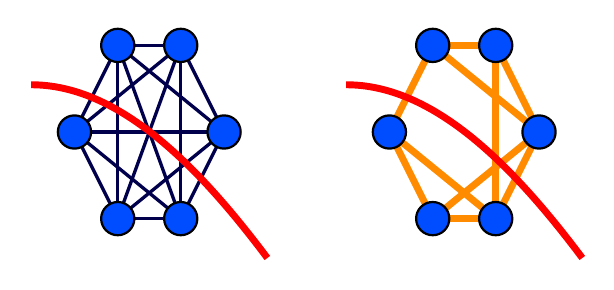
\begin{tikzpicture}[
    vertex/.style={circle, fill=blue!70!cyan, draw=black, line width=0.8pt, minimum size=12pt, inner sep=0pt},
    edge/.style={draw=blue!30!black, line width=1.2pt},
    oedge/.style={draw=orange!90!yellow, line width=2.5pt},
    cut/.style={draw=red, line width=2.5pt}
]
    \def\xsep{4}
    % LEFT: Complete K_6
    \coordinate (L1) at (-0.4, 1.1);  \coordinate (L2) at (0.4, 1.1);
    \coordinate (L3) at (-0.95, 0);   \coordinate (L4) at (0.95, 0);
    \coordinate (L5) at (-0.4, -1.1); \coordinate (L6) at (0.4, -1.1);
    \draw[edge] (L1)--(L2); \draw[edge] (L1)--(L3); \draw[edge] (L1)--(L4);
    \draw[edge] (L1)--(L5); \draw[edge] (L1)--(L6); \draw[edge] (L2)--(L3);
    \draw[edge] (L2)--(L4); \draw[edge] (L2)--(L5); \draw[edge] (L2)--(L6);
    \draw[edge] (L3)--(L4); \draw[edge] (L3)--(L5); \draw[edge] (L3)--(L6);
    \draw[edge] (L4)--(L5); \draw[edge] (L4)--(L6); \draw[edge] (L5)--(L6);
    \node[vertex] at (L1) {}; \node[vertex] at (L2) {};
    \node[vertex] at (L3) {}; \node[vertex] at (L4) {};
    \node[vertex] at (L5) {}; \node[vertex] at (L6) {};
    \draw[cut] (-1.5, 0.6) .. controls (-0.4, 0.6) and (0.6, -0.4) .. (1.5, -1.6);
    % RIGHT: Sparse graph
    \coordinate (R1) at (\xsep-0.4, 1.1);  \coordinate (R2) at (\xsep+0.4, 1.1);
    \coordinate (R3) at (\xsep-0.95, 0);   \coordinate (R4) at (\xsep+0.95, 0);
    \coordinate (R5) at (\xsep-0.4, -1.1); \coordinate (R6) at (\xsep+0.4, -1.1);
    \draw[oedge] (R1)--(R2); \draw[oedge] (R1)--(R3); \draw[oedge] (R2)--(R4);
    \draw[oedge] (R3)--(R5); \draw[oedge] (R4)--(R6); \draw[oedge] (R5)--(R6);
    \draw[oedge] (R3)--(R6); \draw[oedge] (R4)--(R5);
    \draw[oedge] (R1)--(R4); \draw[oedge] (R2)--(R6);
    \node[vertex] at (R1) {}; \node[vertex] at (R2) {};
    \node[vertex] at (R3) {}; \node[vertex] at (R4) {};
    \node[vertex] at (R5) {}; \node[vertex] at (R6) {};
    \draw[cut] (\xsep-1.5, 0.6) .. controls (\xsep-0.4, 0.6) and (\xsep+0.6, -0.4) .. (\xsep+1.5, -1.6);
\end{tikzpicture}
\pause 
\questionbox{What are the cut weights for any $S$?} 
\moveb \pause 
$w_G(\delta S) = |S| \cdot |\overline S|  $ \hfil \pause  
$w_H(\delta S) \approx \frac{d}{n} \cdot \frac{n}{d} \cdot  |S| \cdot |\overline S|  $ 
\[ \forall S \subset V:   \frac{w_G(\delta S)}{w_H(\delta S)} \approx 1 \]
\pause 
\yellbox{Bencz\' ur \& Karger: Can find such $H$ quickly for any $G$!} 
\end{center}
\end{frame}
%%%%%%%%%%%%%%%%%%%%%%%%%%%%
\begin{frame}
\frametitle{Graph Sparsification: What is \alert{good} sparse?}
Recall if $\bff \in \{0,1\}^n$ represents $S$ then $\bff\transpose\bL_{G}\bff = \pause \text{cut}_G(S) $
\pause 
\[
\alert{(1-\eps)} \text{cut}_{H}(S) \leq  \text{cut}_{G}(S) \leq \alert{(1+\eps)} \text{cut}_{H}(S)
\]
\pause 
becomes
\[
\alert{(1-\eps)} \bff\transpose\bL_{H}\bff  \leq  \bff\transpose\bL_{G}\bff  \leq \alert{(1+\eps)}  \bff\transpose\bL_{H}\bff 
\]
\moveb  \pause 
If we ask this only for $\bff \in \{0,1\}^n \to (1+\eps)$-cut similar {\tiny combinatorial}\\
\vskip -0.5em
\notecol{\tiny  \qquad Bencz\' ur \& Karger (1996)} \\
\pause 
If we ask this for all $\bff \in \R^n \to$  \pause \emphcol{$(1+\eps)$-spectrally similar} \\
\vskip -0.5em
\notecol{\tiny  \qquad Spielman \& Teng (2004)} \\
\pause \bigskip 
\yellbox{Spectral sparsifiers are stronger!} \\ \pause 
\notecol{\tiny  \qquad but checking for spectral similarity is easier} 

\end{frame}
%%%%%%%%%%%%%%%%%%%%%%%%%%%%
\MakeLastSlide
\end{document}
